\section{osmo-bts.cfg}\label{Osmo-bts.cfg}
\begin{lstlisting}
!
! OsmoBTS () configuration saved from vty
!!
!
log stderr
  logging color 1
  logging timestamp 0
  logging level rsl info
  logging level oml info
  logging level rll notice
  logging level rr notice
  logging level meas notice
  logging level pag info
  logging level l1c info
  logging level l1p info
  logging level dsp info
  logging level abis notice
!
line vty
 no login
!
phy 0
 instance 0
 osmotrx rx-gain 1
 osmotrx ip local 127.0.0.1
 osmotrx ip remote 127.0.0.1
bts 0
 band PCS1900
 ipa unit-id 1901 0
 oml remote-ip 127.0.0.1
 paging lifetime 0
 gsmtap-sapi bcch
 gsmtap-sapi ccch
 gsmtap-sapi rach
 gsmtap-sapi agch
 gsmtap-sapi pch
 gsmtap-sapi sdcch
 gsmtap-sapi pacch
 gsmtap-sapi pdtch
 gsmtap-sapi sacch
 trx 0
  phy 0 instance 0
\end{lstlisting}


\newpage
\section{openbsc.cfg} \label{Openbsc.cfg}
\begin{lstlisting}
!
! OpenBSC configuration saved from vty
!   !
password foo
!
line vty
 no login
!
e1\_input
 e1\_line 0 driver ipa
 e1\_line 0 port 0
network
 network country code 262
 mobile network code 99
 short name mitm2
 long name mitm2
 auth policy accept-all
 location updating reject cause 13
 encryption a5 0
 neci 1
 paging any use tch 0
 rrlp mode ms-based
 mm info 1
 handover 0
 handover window rxlev averaging 10
 handover window rxqual averaging 1
 handover window rxlev neighbor averaging 10
 handover power budget interval 6
 handover power budget hysteresis 3
 handover maximum distance 9999
 timer t3101 10
 timer t3113 60
 timer t3122 10
 dtx-used 0
 subscriber-keep-in-ram 0
 bts 0
  type sysmobts
  band PCS1900
  cell\_identity 0
  location\_area\_code 1
  training\_sequence\_code 7
  base\_station\_id\_code 63
  ms max power 0
  cell reselection hysteresis 4
  rxlev access min 0
  periodic location update 30
  channel allocator descending
  rach tx integer 9
  rach max transmission 7
  channel-descrption attach 1
  channel-descrption bs-pa-mfrms 5
  channel-descrption bs-ag-blks-res 1
  ip.access unit\_id 1901 0
  oml ip.access stream\_id 255 line 0
  neighbor-list mode automatic
  trx 0
   rf\_locked 0
   arfcn 806
   nominal power 0
   max\_power\_red 0
   rsl e1 tei 0
    timeslot 0
     phys\_chan\_config CCCH+SDCCH4
     hopping enabled 0
    timeslot 1
     phys\_chan\_config TCH/F
     hopping enabled 0
    timeslot 2
     phys\_chan\_config TCH/F
     hopping enabled 0
    timeslot 3
     phys\_chan\_config TCH/F
     hopping enabled 0
    timeslot 4
     phys\_chan\_config TCH/F
     hopping enabled 0
    timeslot 5
     phys\_chan\_config TCH/F
     hopping enabled 0
    timeslot 6
     phys\_chan\_config TCH/F
     hopping enabled 0
    timeslot 7
     phys\_chan\_config TCH/F
     hopping enabled 0
\end{lstlisting}

\newpage
\section{Starten von OsmoBTS}\label{startOsmoBTS}
\begin{figure}[h] %t=top b=bottom h=here p =eigene page
\centering
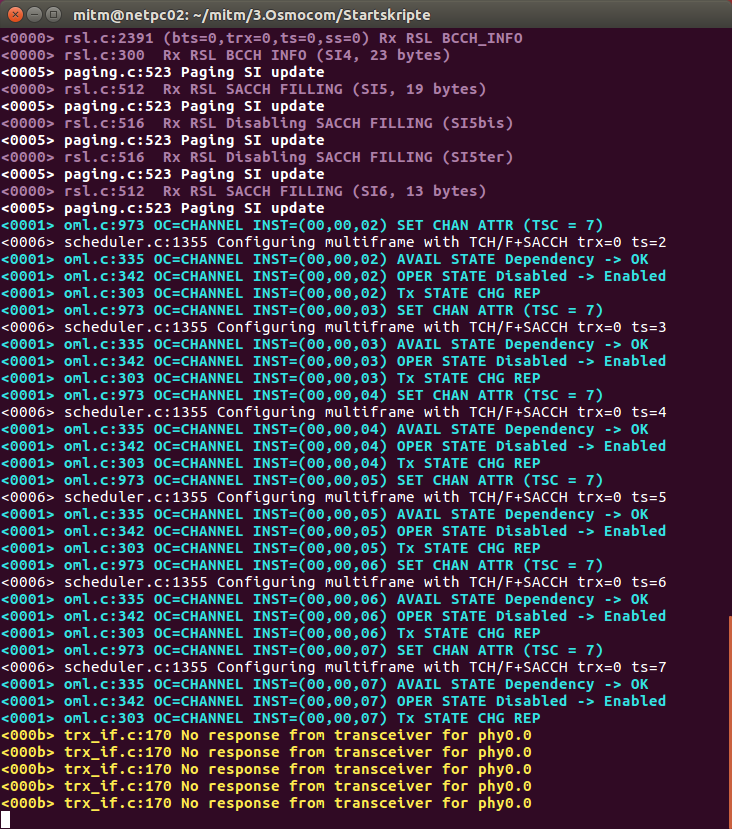
\includegraphics[width=15cm]{includes/Start_OsmoBTS}
\caption{Ansicht der Konsole nach dem Start der OsmoBTS}
\label{fig:OsmoBTS}
\end{figure}

\newpage
\section{Quellcode der GUI-Anwendung}\label{quellcodeGUI}

\textbf{Inhalt von main.cpp}

\begin{lstlisting}
#include "mitm.h"
#include <QApplication>

int main(int argc, char *argv[])
{
    QApplication a(argc, argv);
    MitM w;
    w.show();

    return a.exec();
}
\end{lstlisting}



\vspace{2cm}
\textbf{Inhalt von mitm.h}



\begin{lstlisting}
#ifndef MITM_H
#define MITM_H

#include <QMainWindow>
#include <QProcess>

namespace Ui {
class MitM;
}

class MitM : public QMainWindow
{
    Q_OBJECT

public:
    explicit MitM(QWidget *parent = 0);
    ~MitM();

private:
    Ui::MitM *ui;
    QString password;

public slots:
    void checkInput();
    void transceiverPressed();
    void btsPressed();
    void bscPressed();
    void wiresharkPressed();
    void sipConnectorPressed();
    void sqlBrowserPressed();
    void pcapSipDumpPressed();
    void slot1Pressed();
    void slot2Pressed();
    void slot3Pressed();
    void slot4Pressed();
    void slot5Pressed();
};
#endif // MITM_H
\end{lstlisting}



\vspace{2cm}
\textbf{Inhalt von mitm.cpp}

\begin{lstlisting}
#include "mitm.h"
#include "ui_mitm.h"

MitM::MitM(QWidget *parent) :
    QMainWindow(parent),
    ui(new Ui::MitM)
{
    ui->setupUi(this);

    connect(ui->lineEdit, SIGNAL(textEdited(QString)), this, SLOT(checkInput()));
    connect(ui->pushButtonTransceiver, SIGNAL(clicked()), this, SLOT(transceiverPressed()));
    connect(ui->pushButtonBSC, SIGNAL(clicked()), this, SLOT(bscPressed()));
    connect(ui->pushButtonBTS, SIGNAL(clicked()), this, SLOT(btsPressed()));
    connect(ui->pushButtonSipConnector, SIGNAL(clicked()), this, SLOT(sipConnectorPressed()));
    connect(ui->pushButtonWireshark, SIGNAL(clicked()), this, SLOT(wiresharkPressed()));
    connect(ui->pushButtonSQLBrowser, SIGNAL(clicked()), this, SLOT(sqlBrowserPressed()));
    connect(ui->pushButtonPcap, SIGNAL(clicked()), this, SLOT(pcapSipDumpPressed()));
    connect(ui->pushButtonSlot1, SIGNAL(clicked()), this, SLOT(slot1Pressed()));
    connect(ui->pushButtonSlot2, SIGNAL(clicked()), this, SLOT(slot2Pressed()));
    connect(ui->pushButtonSlot3, SIGNAL(clicked()), this, SLOT(slot3Pressed()));
    connect(ui->pushButtonSlot4, SIGNAL(clicked()), this, SLOT(slot4Pressed()));
    connect(ui->pushButtonSlot5, SIGNAL(clicked()), this, SLOT(slot5Pressed()));
}


MitM::~MitM()
{
    delete ui;
}


void MitM::checkInput() {
    password = ui->lineEdit->text();
}


void MitM::transceiverPressed(){

    QProcess* exec = new QProcess(this);

    if (ui->pushButtonTransceiver->isChecked()) {
        exec->start("./startTransceiver.sh");
        ui->pushButtonTransceiver->setText("Stoppen");
    }
    else {
        exec->close();
        ui->pushButtonTransceiver->setText("Starten");
    }
}



void MitM::bscPressed(){

    QProcess* exec = new QProcess(this);

    if (ui->pushButtonBSC->isChecked()) {
        exec->start("./startOsmoNitb.sh");
        ui->pushButtonBSC->setText("Stoppen");
    }
    else {
        exec->close();
        ui->pushButtonBSC->setText("Starten");
    }
}


void MitM::btsPressed(){

    QProcess* exec = new QProcess(this);

    if (ui->pushButtonBTS->isChecked()) {
        exec->start("./startOsmoBTS.sh");
        ui->pushButtonBTS->setText("Stoppen");
    }
    else {
        exec->close();
        ui->pushButtonBTS->setText("Starten");
    }
}



void MitM::wiresharkPressed(){

    QProcess* exec = new QProcess(this);

    if (ui->pushButtonWireshark->isChecked()) {
        exec->start("./wireshark.sh");
        ui->pushButtonWireshark->setText("Stoppen");
    }
    else {
        exec->close();
        ui->pushButtonWireshark->setText("Starten");
    }
}



void MitM::sipConnectorPressed(){

    QProcess* exec = new QProcess(this);

    if (ui->pushButtonSipConnector->isChecked()) {
        exec->start("./startSipConnector.sh");
        ui->pushButtonSipConnector->setText("Stoppen");
    }
    else {
        exec->close();
        ui->pushButtonSipConnector->setText("Starten");
    }
}



void MitM::sqlBrowserPressed(){

    QProcess* exec = new QProcess(this);

    if (ui->pushButtonSQLBrowser->isChecked()) {
        exec->start("./startSQLBrowser.sh");
        ui->pushButtonSQLBrowser->setText("Stoppen");
    }
    else {
        exec->close();
        ui->pushButtonSQLBrowser->setText("Starten");
    }
}



void MitM::pcapSipDumpPressed(){

    QProcess* exec = new QProcess(this);

    if (ui->pushButtonPcap->isChecked()) {
        exec->start("./startPcapSipDump.sh");
        ui->pushButtonPcap->setText("Stoppen");
    }
    else {
        exec->close();
        ui->pushButtonPcap->setText("Starten");
    }
}


void MitM::slot1Pressed(){
    QProcess* exec = new QProcess(this);
    exec->start("./slot1.sh");
}

void MitM::slot2Pressed(){
    QProcess* exec = new QProcess(this);
    exec->start("./slot2.sh");
}

void MitM::slot3Pressed(){
    QProcess* exec = new QProcess(this);
    exec->start("./slot3.sh");
}

void MitM::slot4Pressed(){
    QProcess* exec = new QProcess(this);
    exec->start("./slot4.sh");
}

void MitM::slot5Pressed(){
    QProcess* exec = new QProcess(this);
    exec->start("./slot5.sh");
}
\end{lstlisting}


\newpage
\section{Installations- und Konfigurations-Skript} \label{configureScript}
\lstinputlisting{../../4.Projektziel-Umsetzung/configureRecord.sh}

\newpage
 \section{Skript zum Starten der Konvertierung} \label{startingConvertScript}
 \lstinputlisting{../../4.Projektziel-Umsetzung/startPcap2wavgsmConversion.sh}
